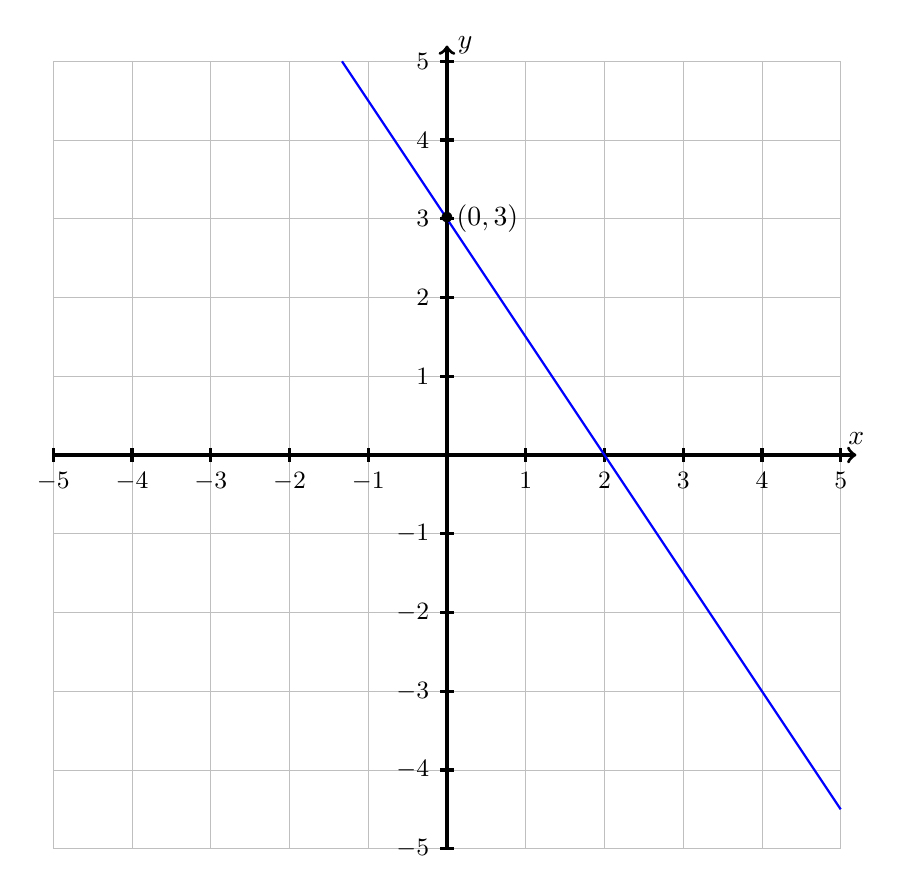
\begin{tikzpicture}
  \def\size{5}
  \path [draw, help lines, opacity=.5]  (-\size,-\size) grid (\size,\size);

  \foreach \i in {1,...,\size} 
  \draw [very thick] (\i,2.5pt) -- +(0,-5pt) node [anchor=north, font=\small] {$\i$}
  (-\i,2.5pt) -- +(0,-5pt) node [anchor=north, font=\small] {$-\i$} 
  (2.5pt,\i) -- +(-5pt,0) node [anchor=east, font=\small] {$\i$}
  (2.5pt,-\i) -- +(-5pt,0) node [anchor=east, font=\small] {$-\i$};
  
  \draw [very thick,->] (-\size,0) -- (\size+.2,0) node [anchor=south] {$x$};
  \draw [very thick,->] (0,-\size) -- (0,\size+.2) node [anchor=west] {$y$};

  \draw [thick, blue] (-4/3,5) -- (5,-4.5);
  \node at (0,3) {$\bullet$};
  \node [right] at (0,3) {$(0,3)$};
  
\end{tikzpicture}
